\documentclass[a0,portrait]{a0poster}
\usepackage{abll-poster}
\usepackage{graphicx}
\usepackage{wrapfig}
\usepackage{nonfloat}
\usepackage{multicol}
\setlength{\columnsep}{75pt}


\definecolor{Shade}{HTML}{F2E6CE}


\newcommand{\Ca}{C$_{\alpha}${}}


\begin{document}
\ULCornerWallPaper{1.0}{figures/ku-background.pdf}
\fontsize{40pt}{60pt}\selectfont

\begin{textblock}{100}(0,0)
\Faculty{\an{department of computer science}}
\\
\Department{\an{university of copenhagen}}
\end{textblock}

\begin{textblock}{100}(0,7)
\Title{Fitting an All-atom Protein Model to a $C_\alpha$-trace}
\end{textblock}

\begin{textblock}{100}(0,12.5)
\Authors{Martin Dybdal, Anders Boesen Lindbo Larsen and Esben Skaarup}
\\[-8mm]
\AuthorEmails{\texttt{dybber@dybber.dk}, \texttt{abll@diku.dk} and \texttt{sben@diku.dk}}
\\[-2mm]
\AuthorEmails{Supervisors: Pawel Winter and Rasmus Fonseca}
\end{textblock}

\linespread{1.075}\fontsize{28pt}{40pt}\selectfont

\renewcommand{\labelitemi}{--\ }

\begin{GridBlock}{0}{21}{100}
\begin{multicols}{3}
%\begin{multicols}{2}
\Head{Summary}

\vspace*{-.4cm}
In this work we investigate a strategy for predicting the structure of proteins. Given a so-called \emph{\Ca-trace}, we wish to fold the protein to match the trace.
%\newpage
\begin{figure}
\vspace{1.7cm}
\hspace{-3cm}
\includegraphics[width=.4\columnwidth]{../rapport/figures/forside.png}
%\hspace{2cm}
\vspace{-1.5cm}
\end{figure}
%\end{multicols}
%\vspace{-.5cm}
%Protein structure prediction can be simplified by using a model that only includes a subset of the atoms present in proteins. In particular, the algorithms group at our department only predicts a folding of the \Ca-trace, and are thus excluding most backbone atoms and all side-chain molecules.



%The strategy divides the problem into two separate tasks.


%\section{Motivation}
%\begin{itemize}
%    \item[-- ] Proteins are the perhaps most important molecules of
%      living organisms.
%    \item[-- ] Computational resolution of the protein 3D-structure has
%      many applications in biotechnology and medicine.
%    \item[-- ] Protein structure prediction and the related topic protein
%      folding, are large and active research fields.
%    \end{itemize}

\section{Our problem}
Currently, we are only able to predict protein structures at the $C_\alpha$-trace level. 
Our goal with this project is to extend the \Ca-trace with the remaining atoms to get an all-atom model.
The difference between the two is shown in Figure \ref{fig:all-atom_vs_trace}.

\begin{figure}
  \centering
  \vspace{1cm}
  \includegraphics[width=0.65\columnwidth]{../rapport/figures/amino_connect}  
  \\[1cm]
  \includegraphics[width=0.65\columnwidth]{../rapport/figures/Calpha_backbone}
  \caption{\textbf{Top}: All-atom protein backbone, with $R_1$, $R_2$ and $R_3$ representing side-chains. \textbf{Bottom}: $C_{\alpha}$-trace. }
  \label{fig:all-atom_vs_trace}
\end{figure}

\section{Our approach}
%The strategy we will pursue, is to use a given $C_\alpha$-trace as target when folding a protein model that contains all atoms. 
The folding should be conducted, such that it minimizes the number of clashes and at the same time minimizes the deviation from the target $C_\alpha$-trace.

We consider our fitting problem as two somewhat separate problems.
First, we fold the backbone to the \Ca-trace.
Hereafter, the amino acid side-chains are added to the backbone.
%In the following we have chosen to
%consider these two tasks separately.
%However, as we shall see in Section \ref{sec:evaluation_handling_side-chains}, the performance of our residue handling depends heavily on the backbone fitting.
 % (even though the residue handling might require us to adjust the backbone).



\end{multicols}
\end{GridBlock}

\begin{GridBlockFill}{0}{44}{100}

  \begin{multicols}{2}
\begin{minipage}{\linewidth} 
    \begin{multicols}{2}
    \Head{Protein Geometry}

    \begin{itemize}
    \item Proteins are built from unbranched chains of amino acids.
    \item All amino acids share
      the same basic structure and a variable side-chain.
    \item The structure of an amino acid can be described by bond lengths,
      bond angles and rotational angles.
    \item The bond lengths and bond angles only displays small variations
      between amino acids (see tables).
    \item Only three different rotational angles occurs along an amino
      acid chain. These are named $\phi$, $\psi$ and $\omega$ and are
      shown on Figure \ref{fig:torsion_angles}.
    \end{itemize} 
   \end{multicols}


\begin{multicols}{2}


\begin{minipage}{\linewidth} 
\centering

  \vspace{7mm}
  \begin{tabular}{lrr}
    \multicolumn{1}{c}{Bond} & \multicolumn{1}{c}{Avg. length} & \multicolumn{1}{c}{Std.dev.} \\ \midrule
    C-O   & 1.2260 Å & 0.0188 Å\\
    CA-C  & 1.5272 Å & 0.0191 Å\\
    N-CA  & 1.4680 Å & 0.0237 Å\\
    C-N   & 1.3234 Å & 0.0215 Å\\
  \end{tabular}
  \vspace{4mm}
  \label{tab:average_bond_lengths}
  \tabcaption{Average bond lengths (in ångstrøm)}
\end{minipage}


\begin{minipage}{\linewidth} 
\centering
  \vspace{7mm}
  \begin{tabular}{lrr}
    \multicolumn{1}{c}{Angle} & \multicolumn{1}{c}{Avg. angle} & \multicolumn{1}{c}{Std.dev.} \\ \midrule 
    H-N-CA & 118.9553$^\circ$ & 1.9979$^\circ$\\
    N-CA-C & 110.6099$^\circ$ & 2.4668$^\circ$\\
    CA-C-N & 116.7804$^\circ$ & 1.7682$^\circ$\\
    C-N-CA & 121.4547$^\circ$ & 1.9946$^\circ$\\
  \end{tabular}
  \vspace{4mm}
  \label{tab:average_bond_angles}
  \tabcaption{Average bond angles}
\end{minipage}

   \end{multicols}
\end{minipage}

\pagebreak

\begin{minipage}{\linewidth} 
\centering% 
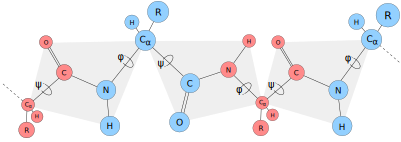
\includegraphics[width=0.90\linewidth, clip=]{figures/protein-torsion-angles.pdf}

\figcaption{Rotational angles in a protein backbone}% 
\label{fig:torsion_angles}
\end{minipage}

\begin{multicols}{2}
  \begin{itemize}
  \item The $\omega$-angle is almost always at $180^{\circ}$, except
    for a few occurrences where it is $0^{\circ}$. To simplify the
    problem, we have assumed that it is always locked at
    $180^{\circ}$.
  \item The $\phi$ and $\psi$ angles are the most variable parts of
    the protein backbone and many models use these as the only
    parameters when performing protein structure prediction.
  \item The $\phi$ and $\psi$ are the only parameters we modify when
    folding the backbone.
  \end{itemize}
\end{multicols}
\end{multicols}



\end{GridBlockFill}

\begin{GridBlock}{0}{72.3}{49}
\begin{multicols}{2}
\Head{Backbone folding}

Given a \Ca-trace, we wish to fold the protein backbone (only the $\phi$ and $\psi$ angles) to match the trace as closely as possible
The backbone fitting problem can be regarded as an \emph{inverse kinematics} problem.
%IK is the process of determining angles of joints in a chain of rigid links in order to make the end of the linked chain reach a desired position in space.
%The end of the the linked chain is called the \emph{end-effector}.


%To simplify the problem, we can separately consider each backbone \Ca\ as an end-effector that must reach its corresponding target \Ca.
%In this way the problem is decomposed into many small IK problems.
%However, this simplification is not entirely valid as the entire backbone cannot be fitted by solving many local problems.
%For example, a configuration of $\phi$ and $\psi$ angles might fit a single \Ca\ to its target, but in such a way that the next \Ca\ in the backbone cannot come close to its target.
%Therefore, a good solution should take global context into account when solving IK problems locally. 

%For the backbone fitting problem we have chosen to experiment with the CCD approach as it is simple, fast, numerically stable and flexible (i.e. it is easy to introduce constraints).

To solve this problem, we have devised an extension to the \emph{cyclic coordinate descent} (CCD) algorithm:
\begin{itemize}
	\item CCD works by adjusting angles one by one in a greedy manner.
	\item We adjust each angle with the goal of minimizing the mean distance between the three forthcoming amino acids $C$ and their corresponding \Ca-targets $T$.
	\item The angles are adjusted iteratively in both directions interchangably until the deviation has converged.
\end{itemize}

\begin{figure}
  \centering
	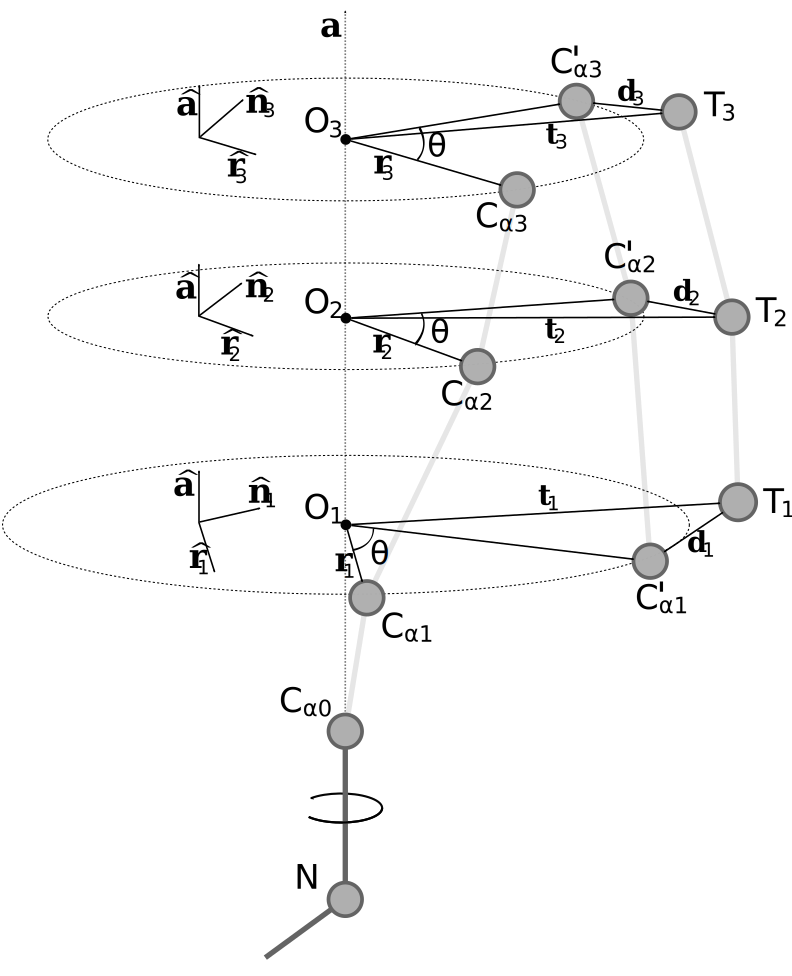
\includegraphics[width=0.85\columnwidth]{../rapport/figures/ccd}
  \caption{Adjusting an angle according to the \Ca-targets with the CCD algorithm.}
  \label{fig:ccd}
\end{figure}
\end{multicols}
\end{GridBlock}



\begin{GridBlock}{51}{72.3}{49}
% \begin{wrapfigure}{r}{0.55\textwidth}
%     \centering
%     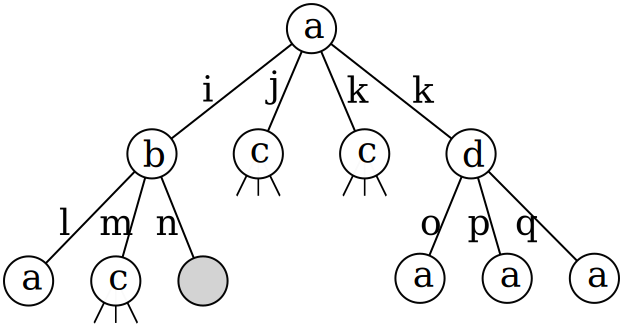
\includegraphics[width=.45\textwidth]{../rapport/figures/rotamersearch}
%     \caption{The structure of our rotamer search space when
%       eliminating collisions with the amino acid \textit{a}.}
%     \label{fig:rotamer-search-tree}
% \end{wrapfigure}
\begin{multicols}{2}
\Head{Rotamer selection} 
\vspace{-4mm}
\begin{itemize}
\item After the backbone is folded in place and fitted to the
  \Ca-trace, we remain with the problem of adding side chains to each
  amino acid.

\begin{minipage}{\linewidth} 
\centering% 
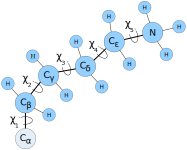
\includegraphics[width=0.90\linewidth, clip=]{../rapport/figures/lysine.pdf}

\figcaption{$\chi$-angles in Lysine side chain}
\label{fig:lysine}
\end{minipage}
\vspace{1mm}
\item The rotational angles of side chains are named
  $\chi_1$-$\chi_5$, but many amino acids only have one or two of
  these angles.

\item Each side chain tends to have certain configurations of its
  $\chi$-angles. These often occuring configurations are called
  rotamers of the side-chain.

\item There exists rotamer libraries containing these common
  configurations together with their likelyhood.

\item We have developed a rotamer search algorithm that minimizes the
  number of occurences, which uses the rotamer-probabilities as a good
  initial guess.
\end{itemize}
\end{multicols}
\end{GridBlock}

%\begin{GridBlock}{51}{80}{48}
%\Head{Conclusion}
%\begin{itemize}
%\item[-- ] We can obtain a RMSD of less than $0.2$ Å with our devised
%  variant of cyclic coordinate descent
%\item[-- ] Selecting the appropriate rotamers makes it possible to
%  reduce the number collisions to 1 for every 4700 amino acids on a
%  realistic protein.
%\end{itemize}
%\end{GridBlock}




\end{document}

